\cleardoublepage
\chapter{Comparison of different arithmetics}
%\label{ch:chapter1}
\label{makereference}
\section{Floating and fixed point arithmetic}

\\
\\
\\
¿DEBO EXPLICAR COMO FUNCIONA CADA UNA DE LAS ARITMÉTICAS?
\\
\\
\\

La aritmética en punto flotante permite realizar operaciones con resolución ¿dinámica, adaptable?. Sin embargo, su implemetación en hardware es mucho mas costosa en términos de recursos, limitando la mayoría de diseños a punto fijo.[lo he sacado de 35]

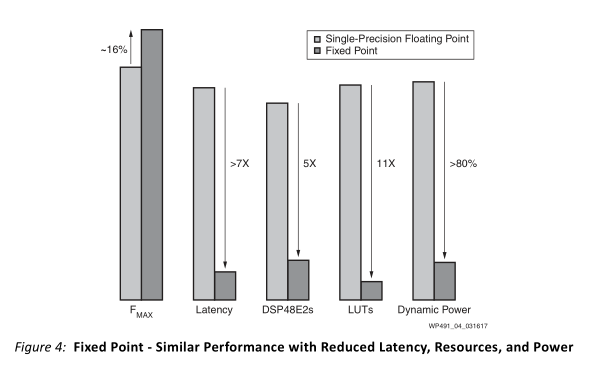
\includegraphics[height=2.5in]{figures/fp_vs_fp.png}
\\
Comparación de los señores de Xilinx. lo he sacado de wp491

\section{Transforming the algorithm into fixed-point}
Una vez hecha la implementación en software se cambiará el tipo de datos de punto flotante a entero con 64 bits. Con este cambio se podrán observar en que pasos del algoritmo se pierde precisión por llegar a los limites representables con enteros con esa resolución -tanto por ser números cercanos al cero como al desbordar por llegar a los valores máximos y mínimos- y se intentará mejorar la precisión desplazando, es decir multiplicando y dividiendo por potencias de dos. (esto o lo explico mejor o meto un apartado antes).
\\
Así, si un valor se acerca a 0 será multiplicado para mantener más precisión y si se encuentra cerca del desbordamiento, será dividido para evitarlo. Al ser los resultados de cada pixel relativos al resto, el orden de ¿anomalidad? no sé ve afectado siempre que estás operaciones se apliquen a todo el conjunto de datos de manera simultanea. Además, estas operaciones resultan triviales en una FPGA.
\\
Conforme se vaya mejorando la precisión, también se irá limitando la cantidad de bits usada con el objetivo de usar menos bits en la fpga y ahorrar lógica. Esto es de especial importancia en los dsp, donde al ser bloques definidos en fabricación, tienen operandos de tamaños fijos. Aquí se muestra una tabla con el número de DSP que necesita una multiplicación según la precisión de sus operandos.
\\
\begin{center}
 \begin{tabular}{||c c c c||} 
 \hline
 Col1 & Col2 & Col2 & Col3 \\ [0.5ex] 
 \hline\hline
 1 & 6 & 87837 & 787 \\ 
 \hline
 2 & 7 & 78 & 5415 \\
 \hline
 3 & 545 & 778 & 7507 \\
 \hline
 4 & 545 & 18744 & 7560 \\
 \hline
 5 & 88 & 788 & 6344 \\ [1ex] 
 \hline
\end{tabular}
\end{center}

Con los datos obtenidos de precisión y de uso de recursos, se elegirá una precisión para cada operación manteniendo estos dos valores en equilibrio.

\section{validación y precisión}
\\
\\
\\
CUANDO PUEDA PONGO UN POCO LO QUE ME HAS DICHO
\\
\\
\\